\section{Wstęp}

\begin{frame}{Kiedy myślimy o dronach...}
    \begin{columns}
        \column{0.5\textwidth}
        Zazwyczaj wyobrażamy sobie operatora z padem w dłoni. 
        \vspace{0.5cm}
        
        Jednak w nowoczesnym przemyśle, ratownictwie i logistyce sterowanie ręczne to przeszłość.
        
        \column{0.5\textwidth}
        \begin{center}
        \begin{tikzpicture}
            \node[inner sep=0pt] (drone) at (0,0) {\includegraphics[width=0.8\textwidth]{example-image-a}}; % Miejsce na obrazek drona/operatora
            \node[below=0.2cm of drone] {Od sterowania do autonomii};
        \end{tikzpicture}
        \end{center}
    \end{columns}
\end{frame}

\begin{frame}{Schemat quadcoptera -- jak to działa?}
    Aby maszyna mogła latać, potrzebuje czterech wirników, które generują ciąg (siłę nośną).
    \vspace{0.5cm}
    
    \begin{center}
    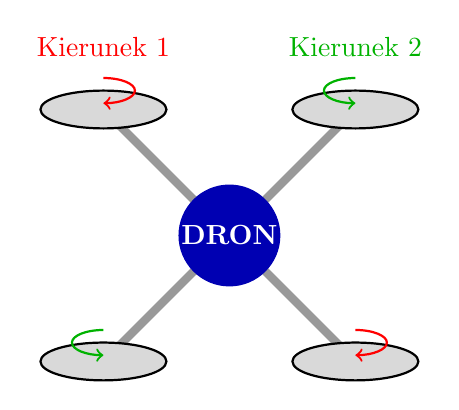
\begin{tikzpicture}[scale=0.8]
        % Ramiona drona
        \draw[line width=3pt, gray!80] (-2,-2) -- (2,2);
        \draw[line width=3pt, gray!80] (-2,2) -- (2,-2);
        
        % Korpus
        \filldraw[blue!70!black] (0,0) circle (0.8cm) node[white, font=\bfseries] {DRON};
        
        % Wirniki (z zaznaczeniem kierunku obrotu)
        % Górny lewy - CW
        \filldraw[gray!30, draw=black, thick] (-2,2) ellipse (1cm and 0.3cm);
        \draw[->, thick, red] (-2, 2.5) arc (90:-90:0.5cm and 0.2cm);
        
        % Górny prawy - CCW
        \filldraw[gray!30, draw=black, thick] (2,2) ellipse (1cm and 0.3cm);
        \draw[->, thick, green!70!black] (2, 2.5) arc (90:270:0.5cm and 0.2cm);
        
        % Dolny lewy - CCW
        \filldraw[gray!30, draw=black, thick] (-2,-2) ellipse (1cm and 0.3cm);
        \draw[->, thick, green!70!black] (-2, -1.5) arc (90:270:0.5cm and 0.2cm);
        
        % Dolny prawy - CW
        \filldraw[gray!30, draw=black, thick] (2,-2) ellipse (1cm and 0.3cm);
        \draw[->, thick, red] (2, -1.5) arc (90:-90:0.5cm and 0.2cm);
        
        % Oznaczenia
        \node[red] at (-2, 3) {Kierunek 1};
        \node[green!70!black] at (2, 3) {Kierunek 2};
    \end{tikzpicture}
    \end{center}
\end{frame}

\begin{frame}{Czym jest autonomia?}
    Autonomia w robotyce oznacza, że maszyna sama podejmuje decyzje i wie:
    \begin{itemize}
        \item Gdzie się znajduje?
        \item Gdzie ma polecieć?
        \item Jak tam dotrzeć, omijając przeszkody?
    \end{itemize}
    \vspace{0.5cm}
    \textbf{Odpowiedzią na te pytania jest matematyka.} Pojęcia z lekcji matematyki i fizyki stają się potężnymi narzędziami, z których korzystają współczesne technologie.
\end{frame}

\begin{frame}{Inżynieria lotu -- Jak drony komunikują się ze światem?}
    Za autonomią stoi skomplikowany, ale bardzo uporządkowany proces komunikacji. 
    Drony porozumiewają się ze stacją naziemną (GCS) za pomocą protokołu \textbf{MAVLink}.
    
    \vspace{0.4cm}
    \begin{center}
    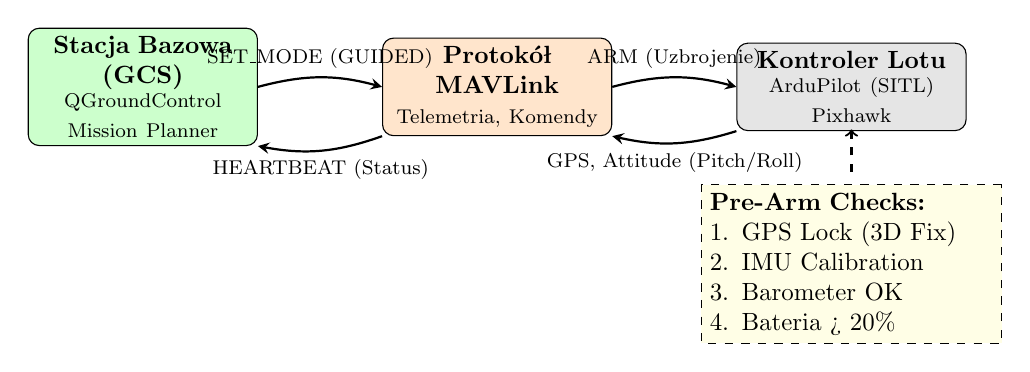
\begin{tikzpicture}[scale=0.9, transform shape,
        box/.style={draw, rounded corners, fill=blue!10, text width=3cm, align=center, minimum height=1.2cm},
        arrow/.style={->, thick, >=stealth}]
        
        % Komponenty
        \node[box, fill=green!20] (gcs) at (0, 0) {\textbf{Stacja Bazowa (GCS)} \\ \footnotesize QGroundControl \\ Mission Planner};
        \node[box, fill=orange!20] (mavlink) at (5, 0) {\textbf{Protokół MAVLink} \\ \footnotesize Telemetria, Komendy};
        \node[box, fill=gray!20] (drone) at (10, 0) {\textbf{Kontroler Lotu} \\ \footnotesize ArduPilot (SITL) \\ Pixhawk};
        
        % Strzałki komunikacji
        \draw[arrow, bend left=15] (gcs.east) to node[above, font=\footnotesize]{SET\_MODE (GUIDED)} (mavlink.west);
        \draw[arrow, bend left=15] (mavlink.east) to node[above, font=\footnotesize]{ARM (Uzbrojenie)} (drone.west);
        
        \draw[arrow, bend left=15] (drone.south west) to node[below, font=\footnotesize]{GPS, Attitude (Pitch/Roll)} (mavlink.south east);
        \draw[arrow, bend left=15] (mavlink.south west) to node[below, font=\footnotesize]{HEARTBEAT (Status)} (gcs.south east);
        
        % Proces Pre-Arm
        \node[draw, dashed, fill=yellow!10, text width=4cm, align=left] at (10, -2.5) {
            \textbf{Pre-Arm Checks:}\\
            1. GPS Lock (3D Fix)\\
            2. IMU Calibration\\
            3. Barometer OK\\
            4. Bateria > 20\%
        };
        \draw[->, dashed, thick] (10, -1.2) -- (10, -0.6);
        
    \end{tikzpicture}
    \end{center}
\end{frame}
